\documentclass[nobib]{tufte-handout}

\usepackage{amssymb}
\usepackage{hyperref}
\usepackage{pgfplots}
\usepackage[activate={true,nocompatibility},final,tracking=true,kerning=true,spacing=true,factor=1100,stretch=10,shrink=10]{microtype}
\usepackage{color}
\usepackage{steinmetz}
\usepackage{placeins}
\usepackage{marginfix}
\usepackage{array}
\usepackage{tikz}
\usepackage{amsmath,amsthm}
\usetikzlibrary{shapes, arrows, positioning, calc}
\usepackage{listings}
\usepackage{forest}
\usepackage{caption}
\usepackage{graphicx}
\usepackage{booktabs}
\usepackage{units}
\usepackage{fancyvrb}
\usepackage{multicol}

\title{ECE 30200 - Probabilistic Methods in Electrical and Computer Engineering}
\author{Zeke Ulrich}

\begin{document}

\maketitle

\tableofcontents

\pagebreak

\section{Background}

The following formulas will be instrumental and may be familar.

\subsection{Series}
\begin{equation}
    \sum_{k=0}^{n} r^k = \frac{1 - r^{n + 1}}{1 - r}
\end{equation}
\begin{equation}
    \sum_{n=1}^{\infty} \frac{1}{n^2} = \frac{\pi^2}{6}
\end{equation}
\begin{equation}
    \sum_{k=1}^{\infty}kr^{k - 1} = \frac{1}{(1 - r)^2}
\end{equation}

\subsection{Combinatorics}
\begin{equation}
    {n\choose k} = \frac{n!}{k!(n - k)!}
\end{equation}
\begin{equation}
    (a + b)^n = \sum_{k=0}^{n} {n\choose k} a^{n - k}b^k
\end{equation}
\begin{equation}
    {n\choose k} + {n\choose k-1} = {n + 1\choose k}
\end{equation}
\begin{equation}
    P(n, k) = \frac{n!}{(n-k)!}
\end{equation}
where $P(n, k)$ is the number of ways to arrange $k$ objects out of $n$ (permutations).
\begin{equation}
    C(n, k) = {n\choose k} = \frac{n!}{k!(n-k)!}
\end{equation}
where $C(n, k)$ is the number of ways to choose $k$ objects out of $n$ (combinations).

\subsection{Approximations}
\begin{align}
    f(x) & = f(a) + f'(a)(x - a) + \frac{f''(a)}{2!}(x - a)^2 + \dots \\
         & = \sum_{n=0}^{\infty} \frac{f^{(n)}(a)}{n!}(x - a)^n
\end{align}
\begin{align}
    1 + x + \frac{x^2}{2!} + \frac{x^3}{3!} + \dots & = \sum_{k=0}^{\infty} \frac{x^k}{k!} \\
                                                    & = e^x
\end{align}
\begin{align}
    \sin(x) & = x - \frac{x^3}{3!} + \frac{x^5}{5!} - \frac{x^7}{7!} + \dots \\
            & = \sum_{n=0}^{\infty} (-1)^n \frac{x^{2n+1}}{(2n+1)!}
\end{align}
\begin{align}
    \cos(x) & = 1 - \frac{x^2}{2!} + \frac{x^4}{4!} - \frac{x^6}{6!} + \dots \\
            & = \sum_{n=0}^{\infty} (-1)^n \frac{x^{2n}}{(2n)!}
\end{align}
\begin{align}
    \ln(1 + x) & = x - \frac{x^2}{2} + \frac{x^3}{3} - \frac{x^4}{4} + \dots \\
               & = \sum_{n=1}^{\infty} (-1)^{n+1} \frac{x^n}{n}
\end{align}

\subsection{Calculus}
\begin{equation}
    \frac{d}{dx} \int_{a}^{x} f(t)\,dt = f(x)
\end{equation}
\begin{equation}
    \int_{a}^{b} f'(x)\,dx = f(b) - f(a)
\end{equation}
\begin{equation}
    \int f(g(x))g'(x)\,dx = \int f(u)\,du
\end{equation}
\begin{equation}
    \int u\,dv = uv - \int v\,du
\end{equation}
\begin{equation}
    \int \frac{1}{(x-a)(x-b)}\,dx = \frac{1}{b-a} \ln\left|\frac{x-a}{x-b}\right| + C
\end{equation}

\subsection{Linear Algebra}
\begin{equation}
    \vec{y} = \beta_1 \vec{x_1} + \beta_2 \vec{x_2} + \cdots + \beta_N \vec{x_N}
\end{equation}
\begin{align}
    \langle \vec{a}, \vec{b} \rangle & = \vec{a}\vec{b}^{T}     \\
                                     & = \sum_{i=1}^{n} a_i b_i
\end{align}
where $\langle \vec{a}, \vec{b} \rangle$ denotes the inner product of vectors $\vec{a}$ and $\vec{b}$.
\begin{equation}
    \|\vec{x}\|_p = \left( \sum_{i=1}^{n} |x_i|^p \right)^{1/p}
\end{equation}
where $\|\vec{x}\|_p$ is the $p$-norm (or $\ell_p$-norm) of vector $\vec{x}$.
\begin{equation}
    \cos(\theta) = \frac{\langle \vec{a}, \vec{b} \rangle}{\|\vec{a}\|_2 \|\vec{b}\|_2}
\end{equation}
where $\theta$ is the angle between vectors $\vec{a}$ and $\vec{b}$.
\begin{equation}
    \hat{\beta} = (\mathbf{X}^T \mathbf{X})^{-1} \mathbf{X}^T \vec{y}
\end{equation}
where $\hat{\beta}$ is the vector of least squares coefficients, $\mathbf{X}$ is the data matrix, and $\vec{y}$ is the target vector

\subsection{Set Theory}
Some important properties of set operations are:
\begin{itemize}
    \item \textbf{Commutativity:}
          \begin{align}
              A \cup B & = B \cup A \\
              A \cap B & = B \cap A
          \end{align}
    \item \textbf{Associativity:}
          \begin{align}
              (A \cup B) \cup C & = A \cup (B \cup C) \\
              (A \cap B) \cap C & = A \cap (B \cap C)
          \end{align}
    \item \textbf{Distributivity:}
          \begin{align}
              A \cup (B \cap C) & = (A \cup B) \cap (A \cup C) \\
              A \cap (B \cup C) & = (A \cap B) \cup (A \cap C)
          \end{align}
    \item \textbf{Identity:}
          \begin{align}
              A \cup \emptyset & = A \\
              A \cap \Omega    & = A
          \end{align}
    \item \textbf{Complement:}
          \begin{align}
              A \cup A^c & = \Omega    \\
              A \cap A^c & = \emptyset
          \end{align}
\end{itemize}

\subsection{Probability Laws}
A probability law must satisfy three axioms:
\begin{enumerate}
    \item Non-negativity: $P(A) \geq 0 \forall A \in F$
    \item Normalization: $P(\Omega) = 1$
    \item Additivity: For any disjoint subsets $\{A_1, A_2, \dots\}$,
          it holds that
          \[P\left[\bigcup_{n=1}^{\infty}A_n\right] = \sum_{n=1}^{\infty}P\left[A_n\right]\]
\end{enumerate}

\subsection{Probability Properties}
\begin{equation}
    P\left[A \cup B\right] = P\left[A\right] + P\left[B\right] - P\left[A \cap B\right]
\end{equation}
\begin{equation}
    P\left[A \cup B\right] \leq P\left[A\right] + P\left[B\right]
\end{equation}
\begin{equation}
    A \subseteq B \implies P\left[A\right] \leq P\left[B\right]
\end{equation}
\section{Formal Definitions}

\subsection{Outcomes}
An \emph{outcome} is the result of some \emph{experiment}.
If that experiment is flipping a coin, the outcome is either
heads or tails. We could express the outcome of heads as $H$,
and the outcome of tails as $T$. The set of all possible
outcomes for an experiment is known as a sample space and is
denoted by $\Omega$. In this case $\Omega = \{H, T\}$.

\subsection{Events}
An \emph{event} $F$ is a subset of the sample space $\Omega$.
The formal definitions of probability are expressed with set
notation. So the event where we have neither heads nor tails is
written as $\{\}$. The event of heads could be expressed as
$\{H\}$, and the event of tails could be expressed as $\{T\}$.
The event of either heads or tails is $\{H, T\}$.

\subsection{Probability Laws}
A \emph{probability law} is a function $P$ that maps an event $A$
to a real number in $[0, 1]$. For the coin example, the probability
law might be $P(\{\}) = 0$, $P(\{H\}) = 0.5$, $P(\{T\}) = 0.5$, and
$P(\{\Omega\}) = 1$. A probability law must satisfy three axioms:
\begin{enumerate}
    \item Non-negativity: $P(A) \geq 0 \forall A \in F$
    \item Normalization: $P(\Omega) = 1$
    \item Additivity: For any disjoint subsets $\{A_1, A_2, \dots\}$,
          it holds that
          \[P\left[\bigcup_{n=1}^{\infty}A_n\right] = \sum_{n=1}^{\infty}P\left[A_n\right]\]
\end{enumerate}

\subsection{Probability Space}
A probability space is a triplet $\Omega, F, P$.

\subsection{Probability Properties}
\begin{equation}
    P\left[A \cup B\right] = P\left[A\right] + P\left[B\right] - P\left[A \cap B\right]
\end{equation}
\begin{equation}
    P\left[A \cup B\right] \leq P\left[A\right] + P\left[B\right]
\end{equation}
\begin{equation}
    A \subseteq B \implies P\left[A\right] \leq P\left[B\right]
\end{equation}
\begin{equation}
    P\left[A | B\right] = \frac{P[A \cap B]}{P[B]}
\end{equation}

Outcomes are statistically \emph{independent} if
$P(A|B) = P(A)$ (assuming P(B) > 0), or
equivalently $P(A \cap B) = P(A)P(B)$.

A \emph{random variable} $X$ is a function $X : \Omega \implies \Re$
that maps an outcome $\epsilon \in \Omega$ to a number $X(\epsilon)$ on the real line.
We call it a variable because it has multiple states. The mapping $X$

\emph{Bayes Theorem} states that for any two events $A$ and $B$ such that $P[A] > 0$ and
$P[B] > 0$,
\begin{equation}
    P[A|B] = \frac{P[B|A]P[A]}{P[B]}
\end{equation}

The \emph{Law of Total Probability} states that if
$\{A_1, A_2, \dots, A_n\}$ is a partition of $\Omega$,
then for any $B \subseteq \Omega$,
\begin{equation}
    P[B] = \sum_{i = 1}^{n} P[B|A_i]P[A_i]
\end{equation}
\section{Discrete Random Variables}

A \emph{random variable} $X$ is a function $X : \Omega \implies \Re$
that maps an outcome $\epsilon \in \Omega$ to a number $X(\epsilon)$ on the real line.
We call it a variable because it has multiple states.

The \emph{expectation} of a random variable $X$ is
\begin{equation}
    E[X] = \sum_{x\in X(\Omega)} xp_X(x)
\end{equation}
The difference between $E[X]$ and the mean is
that $E[X]$ is computed from the ideal histogram,
while mean is computed from the empirical histogram.
In general for any functions $g$ and $h$,
\begin{align}
    E[g(X)]        & = \sum_{x} g(x)p_X(x) \\
    E[g(X) + h(X)] & = E[g(X)] + E[h(X)]   \\
    E[cX]          & = cE[X]               \\
    E[X + c]       & = E[X] + c
\end{align}

The \emph{variance} of a random variable $X$ is
\begin{equation}
    Var[X] = E\left[(X-\mu)^2\right]
\end{equation}
or alternatively, the second moment
minus the first moment squared.
\begin{equation}
    E[X^2] - E[X]^2
\end{equation}

The \emph{probability mass function} (PMF) $p_X(a)$
of a random variable $X$ specifies the probability of
obtaining a number $X(\epsilon) = a$. We denote a PMF as
\begin{equation}
    p_X(a) = P[X = a]
\end{equation}
PMFs are represented with histograms.
\begin{figure}[h]
    \centering
    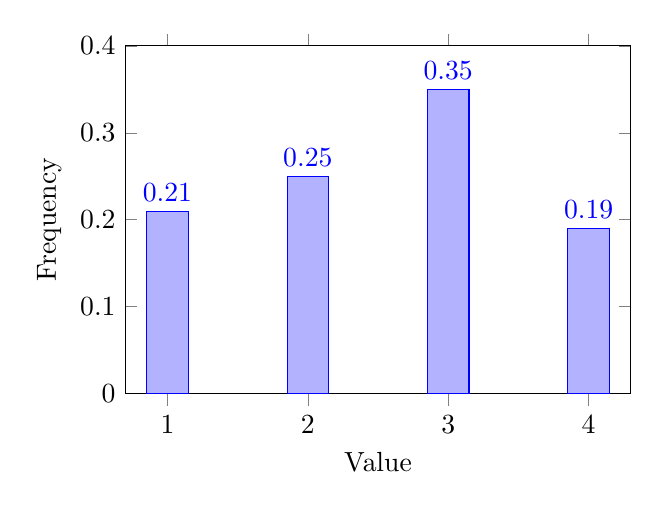
\begin{tikzpicture}
        \begin{axis}[
                ybar,
                bar width=15pt,
                xlabel={Value},
                ylabel={Frequency},
                xtick=data,
                ymin=0,
                ymax=0.4,
                nodes near coords,
                width=8cm,
                height=6cm
            ]
            \addplot coordinates {(1,0.21) (2,0.25) (3,0.35) (4,0.19)};
        \end{axis}
    \end{tikzpicture}
    \caption{PMF}
\end{figure}
A PMF should satisfy
\begin{equation}
    \sum_{x\in X(\Omega)} p_X(x) = 1
\end{equation}

The \emph{cumulative distribution function} is given by
\begin{align}
    F_X(x) & = P\left[X \leq x\right] \\
           & = \sum_{u \leq x} p_X(u)
\end{align}
and represents the sum of every impulse
of the PMF up to $x$.

A \emph{Bernoulli random variable} has a state
of either 0 or 1. The probability of getting 1 is $p$ and
the probability of getting 0 is $1 - p$. We write
\begin{equation}
    X \sim Bernoulli(p)
\end{equation}
or
\begin{equation}
    X \sim B(p)
\end{equation}
to say that $X$ is drawn from a Bernoulli distribution
with a parameter $p$. For a Bernoulli distribution,
\begin{align}
    E[X]   & = p        \\
    E[X^2] & = p        \\
    Var[X] & = p(1 - p)
\end{align}
Say $S \sim B(1-p)$.
Let
\begin{align}
    P(R=0|S=0) & = 1 - \epsilon_0 \\
    P(R=1|S=0) & = \epsilon_0
\end{align}
then $R|S=0 \sim B(\epsilon_0)$.
Let
\begin{align}
    P(R=0|S=1) & = \epsilon_1     \\
    P(R=1|S=0) & = 1 - \epsilon_1
\end{align}
then $R|S=0 \sim B(1 - \epsilon_1)$.
Overall,
\begin{equation}
    R|S \sim B(\epsilon_0^{1-S}(1-\epsilon_1)^S)
\end{equation}

A \emph{Rademacher random variable} has two states, -1 and 1.
The probability of getting each is 0.5.

A \emph{binomial random variable} has a PMF of
\begin{equation}
    p_X(k) = {n\choose k} p^k (1 - p)^{n - k}, k = 0, 1, \dots n
\end{equation}
where $0 < p < 1$ is the binomial parameter, and $n$ is the total
number of states. We write
\begin{equation}
    X \sim Binomial(n, p)
\end{equation}
to say that $X$ is drawn from a binomial distribution with a
parameter $p$ of size $n$.
If $X \sim Binomial(n, p)$, then
\begin{align}
    E[X]   & = np               \\
    E[X^2] & = np(np + (1 - p)) \\
    Var[X] & = np(1 - p)
\end{align}

Let $X$ be a \emph{geometric random variable}. Then the
PMF of $X$ is
\begin{equation}
    p_X(k) = (1 - p)^{k - 1}p, k=1,2,\dots
\end{equation}
We write
\begin{equation}
    X \sim Geometric(p)
\end{equation}
to say that $X$ was drawn from a geometric
distribution with a parameter $p$.
If $X \sim Geometric(p)$ then
\begin{align}
    E[X]   & = \frac{1}{p}                 \\
    E[X^2] & = \frac{2}{p^2} - \frac{1}{p} \\
    Var[X] & = \frac{1 - p}{p^2}
\end{align}

Let $X$ be a \emph{Poisson random variable}. Then the PMF
of $X$ is
\begin{equation}
    p_X(k) = \frac{\lambda^k}{k!}e^{-\lambda}, k=0, 1, 2,\dots
\end{equation}
where $\lambda > 0$ is the Poisson rate. We write
$X \sim Poisson(\lambda)$ to say that $X$ was drawn from
a Poisson distribution with a parameter $\lambda$.
If $X \sim Poisson(\lambda)$ then
\begin{align}
    E[X]   & = \lambda             \\
    E[X^2] & = \lambda + \lambda^2 \\
    Var[X] = \lambda
\end{align}
For small $p$ and large $n$,
\begin{equation}
    {n\choose k}p^k(1-p)^{n-k} \approx \frac{\lambda^k}{k!}e^{-\lambda}
\end{equation}

\emph{Joint Distributions} are higher-dimensional
PDFs, PMFs, or CDFs. We write
\begin{equation}
    f_{X_1, X_2, \dots, X_n}(x_1, x_2, \dots, x_n) \equiv f_{\vec{X}}(\vec{x})
\end{equation}

The \emph{joint PMF} of two random variables
$X$ and $Y$ is notated by
\begin{equation}
    p_{X,Y}(x,y)=P[X=x \text{ and } Y=y]
\end{equation}
and represents the probability of both.

A \emph{marginal PMF} is defined as
\begin{equation}
    p_X(x) = \sum_{y\in \Omega_Y} p_X(x,y)
\end{equation}
or w.l.o.g.
\begin{equation}
    p_Y(y) = \sum_{x\in \Omega_X} p_X(x,y)
\end{equation}
That is, it is the joint PMF summed over
one of the variables.

The \emph{conditional PMF} is given by
\begin{equation}
    p_{X|Y}(x|y) = \frac{p_{X,Y}(x,y)}{p_{Y}(y)}
\end{equation}

If two random variables $X$ and $Y$ are independent,
then
\begin{align}
    p_{X,Y}  & = p_X(x)p_Y(y) \\
    f_{X, Y} & = f_X(x)f_Y(y)
\end{align}
If a sequence of random variables
$X_1, X_2, \dots, X_N$ are independent,
then their joint PDF (or joint PMF) can be
factorized as
\begin{equation}
    f_{X_1,X_2,\dots,X_N}\left(x_1,x_2,\dots,x_N\right) = \prod_{n=1}^{N}f_{X_n}(x_n)
\end{equation}

The \emph{joint CDF} of two random variables
$X$ and $Y$ is the function $F_{X,Y}(x,y)$ such
that
\begin{equation}
    F_{X,Y}(x,y) = P\left[X \leq x \cap Y \leq y\right]
\end{equation}
If $X$ and $Y$ are discrete, then
\begin{equation}
    F_{X,Y}(x,y) = \sum_{y'\leq y}\sum_{x' \leq x} p_{X,Y}(x',y')
\end{equation}

For two random variables $X$ and $Y$,
the \emph{marginal CDF} is
\begin{align}
    F_X(x) & = F_{X,Y}(x, \infty) \\
    F_Y(y) & = F_{X,Y}(\infty, y)
\end{align}

Let $X$ and $Y$ be two random variables.
The \emph{joint expectation} is
\begin{equation}
    E[XY] = \sum_{y\in \Omega_Y}\sum_{x\in \Omega_X}xy \times p_{X,Y}(x,y)
\end{equation}
If $X$ and $Y$ are discrete, then joint
expectation is also called \emph{correlation}.
This can be written in matrix form as
\begin{equation}\label{eq:p}
    \begin{bmatrix}
        p_{X,Y}(x_1, y_1) & p_{X,Y}(x_1, y_2) & \dots  & p_{X,Y}(x_1, y_N) \\
        p_{X,Y}(x_2, y_1) & p_{X,Y}(x_2, y_2) & \dots  & p_{X,Y}(x_2, y_N) \\
        \vdots            & \vdots            & \ddots & \vdots            \\
        p_{X,Y}(x_N, y_1) & p_{X,Y}(x_N, y_2) & \dots  & p_{X,Y}(x_N, y_N)
    \end{bmatrix}
\end{equation}
then the joint expectation is
\begin{equation}
    E[XY] = \sum_{i=1}^{N}\sum_{j=1}^{N}x_i y_j \times p_{X,Y}(x_i, y_j)
\end{equation}
Let the matrix in Equation \ref{eq:p} be $\mathbf{P}$.
Let
\begin{align}
    \vec{x} & = \begin{bmatrix}
                    x_1    \\
                    x_2    \\
                    \vdots \\
                    x_N
                \end{bmatrix} \\
    \vec{y} & = \begin{bmatrix}
                    y_1    \\
                    y_2    \\
                    \vdots \\
                    y_N
                \end{bmatrix}
\end{align}
then
\begin{align}
    E[XY] & = \begin{bmatrix}
                  x_1   &
                  x_2   &
                  \dots &
                  x_N
              \end{bmatrix}
    \begin{bmatrix}
        p_{X,Y}(x_1, y_1) & p_{X,Y}(x_1, y_2) & \dots  & p_{X,Y}(x_1, y_N) \\
        p_{X,Y}(x_2, y_1) & p_{X,Y}(x_2, y_2) & \dots  & p_{X,Y}(x_2, y_N) \\
        \vdots            & \vdots            & \ddots & \vdots            \\
        p_{X,Y}(x_N, y_1) & p_{X,Y}(x_N, y_2) & \dots  & p_{X,Y}(x_N, y_N)
    \end{bmatrix}
    \begin{bmatrix}
        y_1    \\
        y_2    \\
        \vdots \\
        y_N
    \end{bmatrix}                         \\
          & = \vec{x}^T \mathbf{P} \vec{y}
\end{align}
$E[XY]$ is a weighted inner product between the
states. $\vec{x}$ and $\vec{y}$ are the states of
the random variables $X$ and $Y$. Recalling that the
magnitude of the inner product of $\vec{a}$ and $\vec{b}$
is $|a||b|\cos(\theta)$ and that cosine is bounded, we have
\begin{equation}
    -1 \leq \frac{E[XY]}{\sqrt{E[X^2]}\sqrt{E[Y^2]}} \leq 1
\end{equation}
Notice that the correlation of $X,Y$ is
proportional to the covariance.

The covariance of two random variables is
\begin{equation}
    \text{Cov}(X, Y) = E[XY] - E[X]E[Y]
\end{equation}
While $\rho$ is
\begin{equation}
    \rho = \frac{\text{Cov}(X, Y)}{\sqrt{\text{Var}(X)\text{Var}(Y)}}
\end{equation}
\section{Continuous Random Variables}

A \emph{continuous random variable} is
analogous to the discrete case. Recall that
a probability is just a size of a set.
It's easy to find the size of a discrete set
because you can just count elements, but for
an uncountable set new methods are needed. Luckily
the intution for continuous random variables is
intuitive, it's still just the size of a set $A$
relative to $\Omega$.
\begin{figure}[h]
    \centering
    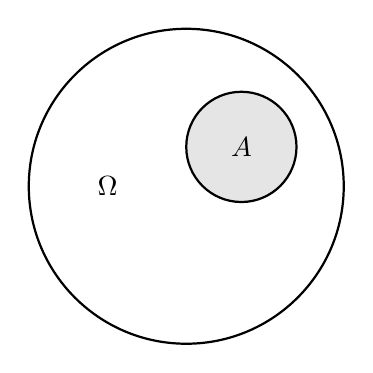
\begin{tikzpicture}[scale=1]
        \draw[thick] (0,0) circle (2cm);
        \node at (-1,0) {$\Omega$};
        \draw[thick, fill=gray!20] (0.7,0.5) circle (0.7cm);
        \node at (0.7,0.5) {$A$};
    \end{tikzpicture}
    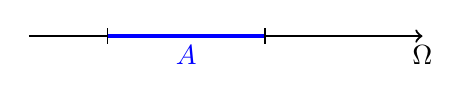
\begin{tikzpicture}[scale=1]
        \draw[thick,->] (0,0) -- (5,0);
        \node[below] at (5,0) {$\Omega$};
        \draw[very thick,blue] (1,0) -- (3,0);
        \node[below,blue] at (2,0) {$A$};
        \draw (1,0.1) -- (1,-0.1);
        \draw (3,0.1) -- (3,-0.1);
    \end{tikzpicture}
    \caption{Continuous random variables}
\end{figure}
Formally, if each event in A is equally likely, then
\begin{equation}
    P[\{x \in A\}] = \frac{\int_{A}dx}{|\Omega|}
\end{equation}
If we relax the assumption of equiprobability, then
more generally
\begin{equation}
    P[\{x\in A\}] = \int_{A} f_X(x) dx
\end{equation}
$f_X(x)$ is called the \emph{probability density function} (PDF).
It is analogous to the probability mass function.

Formally, a probability density function
is a mapping $f_X: \Omega \implies \Re$,
with the following properties:
\begin{itemize}
    \item Non-negativity: $f_X(x) \geq 0 \forall x \in \Omega$
    \item Unity: $\int_{\Omega} f_X(x)dx = 1$
    \item Measure of a set: $P[\{x \in A\}] = \int_{A}f_X(x) dx$
\end{itemize}

We can express a PDF in terms of a PMF
with a train of delta functions like so:
\begin{equation}
    f_X(x) = \sum_{x_k \in \Omega} p_X(x_k) \delta(x - x_k)
\end{equation}

We can also define the probability density
function as the derivative of the CDF, like so:
\begin{equation}
    f_X(x) = \frac{d}{dx}p(X \leq x)
\end{equation}

The expectation of a continuous random variable is
\begin{equation}
    E[X] = \int_{\Omega} xf_X(x)dx
\end{equation}

Properties of the expectation for continuous
random variables:
\begin{itemize}
    \item $E[aX] = aE[X]$
    \item $E[X+a] = E[X] + a$
    \item $E[aX+b] = aE[X] + b$
\end{itemize}

A random variable $X$ has an expectation
if it is absolutely integrable,
\begin{equation}
    E[|X|] = \int_{\Omega} |x|f_X(x)dx < \infty
\end{equation}

The variance of a continuous random variable
$X$ is
\begin{align}
    Var[X] & = E[(X-\mu)^2]                    \\
           & = \int_{\Omega} (x-\mu)^2f_X(x)dx \\
           & = E[X^2] - \mu^2
\end{align}

A continuous \emph{uniform random variable}
has a PDF of
\begin{equation}
    f_X(x) = \begin{cases}
        \frac{1}{b-a} & a \leq x \leq b \\
        0             & \text{else}
    \end{cases}
\end{equation}
We write
\begin{equation}
    X \sim Uniform(a,b)
\end{equation}
to mean that $X$ is drawn from a uniform
distribution on an interval $[a, b]$.
It has a CDF given by
\begin{equation}
    F_X(x) = \begin{cases}
        0               & x < a           \\
        \frac{x-a}{b-a} & a \leq x \leq b \\
        1               & x > b
    \end{cases}
\end{equation}
If $X \sim Uniform(a,b)$ then
\begin{align}
    E[X]   & = \frac{a + b}{2}      \\
    Var[X] & = \frac{(b - a)^2}{12}
\end{align}

A continuous \emph{exponential random variable}
has a PDF of
\begin{equation}
    f_X(x) = \begin{cases}
        \lambda e^{-\lambda x} & x \geq 0    \\
        0                      & \text{else}
    \end{cases}
\end{equation}
\marginnote{An exponential random variable
    is the interarrival time between two consecutive
    Poisson events}
We write
\begin{equation}
    X \sim Exponential(\lambda)
\end{equation}
to mean that $X$ is drawn from an
exponential distribution of parameter
$\lambda$. It has a CDF given by
\begin{equation}
    F_X(x) = 1 - e^{-\lambda x}
\end{equation}
If $X \sim Exponential(\lambda)$, then
\begin{align}
    E[X]   & = \frac{1}{\lambda}   \\
    Var[X] & = \frac{1}{\lambda^2}
\end{align}
Consider $X_n \sim \text{Exponential}(\lambda)$, and let
$X_1, \dots, X_N$ be i.i.d. copies. Define
$Z_N = \sum_{n=1}^{N} X_n$. Then
\begin{equation}
    E[Z_N] = \frac{N}{\lambda}
\end{equation}
and
\begin{equation}
    \text{Var}[Z_N] = \frac{N}{\lambda^2}
\end{equation}


A \emph{Gaussian random variable} is a
random variable $X$ such that its PDF
is
\begin{equation}
    f_X(x) = \frac{1}{\sqrt{2\pi \sigma^2}}\exp\left(-\frac{(x-\mu)^2}{2\sigma^2}\right)
\end{equation}
We write
\begin{equation}
    X \sim Gaussian(\mu, \sigma^2)
\end{equation}
or
\begin{equation}
    X \sim \mathcal{N}\left(\mu, \sigma^2\right)
\end{equation}
to mean that $X$ is drawn from a Gaussian
of parameter $(\mu, \sigma^2)$.
If $X \sim \mathcal{N}(\mu, \sigma^2)$, then
\begin{align}
    E[X]   & = \mu      \\
    Var[X] & = \sigma^2
\end{align}

The \emph{standard Gaussian} random variable has a
PDF given by
\begin{equation}
    f_X(x) = \frac{1}{\sqrt{2\pi}} e^{-\frac{x^2}{2}}
\end{equation}
The CDF of the standard Gaussian is defined
as the $\Phi$ function.
\begin{equation}
    \Phi(x) = \frac{1}{\sqrt{2\pi}}\int_{-\infty}^{\infty} e^{-\frac{t^2}{2}}dt
\end{equation}
The CDF of the standard Gaussian is related to the
\emph{error function}, which is defined as
\begin{equation}
    \text{erf}(x) = \frac{2}{\sqrt{\pi}} \int_{0}^{x} e^{-t^2} dt
\end{equation}
by the relation
\begin{equation}
    \Phi(x) = \frac{1}{2} \left(1 + \text{erf}\left(\frac{x}{\sqrt{2}}\right)\right)
\end{equation}
The CDF of an arbitrary Gaussian is related via
the transformation
\begin{equation}
    F_X(x) = \Phi\left(\frac{x - \mu}{\sigma}\right)
\end{equation}
Let $X \sim \mathcal{N}(\mu, \sigma^2)$, then
\begin{itemize}
    \item $\Phi(y) = 1 -\Phi(-y)$
    \item $P[X\geq b] = 1 - \Phi(\frac{b-\mu}{\sigma})$
    \item $P[|X| \geq b] = 1 - \Phi(\frac{b-\mu}{\sigma}) + \Phi(\frac{-b-\mu}{\sigma})$
\end{itemize}

In addition to mean and variance, we introduce
two more useful quantities, \emph{skewness} and
\emph{kurtosis}.
\begin{align}
    E\left[X\right]                                   & = \mu      \\
    E\left[(X - \mu)^2\right]                         & = \sigma^2 \\
    E\left[\left(\frac{X-\mu}{\sigma}\right)^3\right] & = \gamma   \\
    E\left[\left(\frac{X-\mu}{\sigma}\right)^4\right] & = \kappa
\end{align}
\marginnote{\emph{Excess kurtosis} is defined
    as $\kappa - 3$}

Skewness measures the asymmetry of a
distribution. A Gaussian distribution has
skewness 0. Kurtosis measures how heavy-tailed
the distribution is. If the kurtosis is
positive, then the tails decay faster than a
Gaussian. If the kurtosis is negative, then
the distribution has a tail that
decays more slowly than a Gaussian.

The definition of a CDF is
\begin{equation}
    F_X(x) = P[X \leq x]
\end{equation}
\begin{figure}
    \centering
    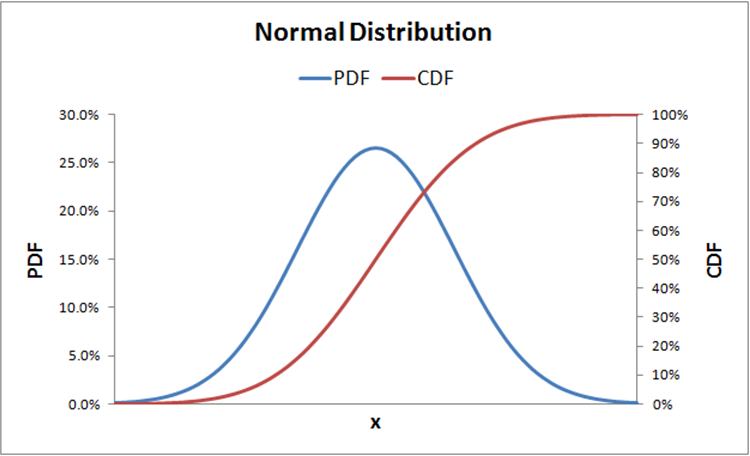
\includegraphics[scale=0.5]{images/normal_distribution_plot.png}
    \caption{PDF and CDF}
\end{figure}
Let $X$ be a continuous random variable. if the CDF
$F_X$ is continuous at any $a\leq x \leq b$, then
\begin{equation}
    P[a \leq X \leq b] = F_X(b) - F_X(a)
\end{equation}
A function $F_X(x)$ is said to be left
continuous if at $x=b$
\begin{equation}
    F_X(b) = \lim_{h\implies 0} F_X(b-h)
\end{equation}
and right continuous if
\begin{equation}
    F_X(b) = \lim_{h\implies 0} F_X(b+h)
\end{equation}
and continuous if $F_X(x)$ is both left
and right continuous.
All CDFs are right continuous.

For any random variable $X$, discrete or continuous,
\begin{equation}
    P[X=b] = \begin{cases}
        F_X(b) - F_X(b^-) & \text{if $F_X$ is discontinuous at $x=b$} \\
        0                 & \text{else}
    \end{cases}
\end{equation}

The PDf is the derivative of the CDF.
\begin{equation}
    f_X(x) = \frac{d}{dx} \int_{-\infty}^{x} f_X(t)dt
\end{equation}
provided $F_X$ is differentiable at $x$. If not, then
\begin{equation}
    f_X(x) = F_X(x) - \lim_{h\implies 0} F_X(x-h)
\end{equation}

Let $X$ be a continuous random variable with PDF
$f_X$. The median of $X$ is a point $c \in \Re$ such that
\begin{equation}
    \int_{-\infty}^{c} f_X(x) dx = \int_{c}^{\infty}f_X(x) dx
\end{equation}

Let $X$ be a continuous random variable. The mode is
the point $c$ such that $f_X(x)$ attains the maximum.
\begin{equation}
    x = \text{argmax}_{x \in \Omega} f_X(x)
\end{equation}

The mean $E[X]$ can be computed from
$F_X$ as
\begin{equation}
    E[X] = \int_{0}^{\infty} (1-F_X(t))dt
\end{equation}

Recall that joint distributions are
higher-dimensional PDFs, PMFs, or CDFs.
\begin{equation}
    f_{\textbf{X}}(\vec{x}) = f_{X_1, \dots, X_N}(x_1, \dots, x_n)
\end{equation}
Let $X$ and $Y$ be two continuous random variables.

The \emph{joint PDF} of $X$ and $Y$ is a function
$f_{X,Y}(x,y)$ that can be integrated to yield a probability
\begin{equation}
    P[A] = \int_{A} f_{X,Y}(x,y)dxdy
\end{equation}
for any event $A \subseteq \Omega_X \times \Omega_Y$.

The \emph{marginal PDF} is defined as
\begin{equation}
    f_X(x) = \int_{\Omega_Y} f_{X,Y}(x,y)dy
\end{equation}
and
\begin{equation}
    f_Y(y) = \int_{\Omega_X} f_{X,Y}(x,y)dx
\end{equation}

The \emph{marginal CDF is}
\begin{align}
    F_X(x) & = F_{X,Y}(x, \infty) \\
    F_Y(y) & = F_{X,Y}(\infty, y)
\end{align}

Let $F_{X,Y}(x,y)$ be the joint CDF of $X$ and $Y$.
Then the joint PDF can be obtained through
\begin{equation}
    f_{X,Y}(x,y) = \frac{\partial^2}{\partial_y\partial_x} F_{X,Y}(x,y)
\end{equation}

If two random variables are \emph{independent},
then
\begin{equation}
    p_{X,Y}(x,y) = p_X(x)p_Y(y)
\end{equation}
and
\begin{equation}
    f_{X,Y}(x,y) = f_X(x)f_Y(y)
\end{equation}

If a sequence of random variables
$X_1, \dots, X_N$ are independent,
then their joint PDF can be factorized.
\begin{equation}
    f_{X_1,\dots,X_N}(x_1,\dots,x_n) = \prod_{n=1}^{N}f_{X_n}(x)n
\end{equation}

A collection of random variables $X_1, \dots, X_N$ are called
\emph{independent and identically distributed} (i.i.d.) if
all are independent and have the same distribution, i.e.
$f_{X_1}(x) = \dots = f_{X_N}(x)$.

The \emph{joint expectation} is
\begin{equation}
    E[XY] = \int_{y\in \Omega_y}\int_{x\in \Omega_x} xy f_{X,Y}(x,y)dxdy
\end{equation}

For an arbitrary $g(X,Y)$,
\begin{equation}
    E[g(X,Y)] = \int_{y\in \Omega_y}\int_{x\in \Omega_x} g(x,y) f_{X,Y}(x,y)dxdy
\end{equation}

Recall
\begin{equation}
    \text{Cov}(X,Y) = E[XY] - E[X]E[Y]
\end{equation}
and now we also state that
\begin{equation}
    \text{Var}[X+Y] = \text{Var}[X] + 2\text{Cov}(X,Y) + \text{Var}[Y]
\end{equation}
We also state that covariance is zero, then so is the correlation.
However if the correlation is zero, the covariance is not necesarily zero.
\begin{equation}
    \text{Cov}(X,Y) = 0 \implies \text{Corr}(X,y) = 0
\end{equation}

If $X$ and $Y$ are independent, then
\begin{equation}
    E[XY] = E[X]E[Y]
\end{equation}
This implies that $X$ and $Y$ are
uncorrelated (i.e. $\text{Cov}(X,Y) = 0$),
but the converse is not true.

Let $X$ and $Y$ be two continuous random variables.
The \emph{conditional PDF} of $X$ given $Y$ is
\begin{equation}
    f_{X|Y}(x|y) = \frac{f_{X,Y}(x,y)}{f_Y(y)}
\end{equation}

Let $X$ and $Y$ be continuous random variables and
$A$ be an event. Then
\begin{equation}
    P[X \in A | Y=y] = \int_{A} f_{X|Y}(x|y)dx
\end{equation}
\begin{equation}
    P[X\in A] = \int_{\Omega_Y} P[X\in A|Y = y]f_Y(y)dy
\end{equation}

The \emph{conditional expectation} of $X$ given $Y=y$ is
\begin{equation}
    E[X|Y=y] = \int_{-\infty}^{\infty}xf_{X|Y}(x|y)dx
\end{equation}

The \emph{law of total expectation} is
\begin{equation}
    E[X] = \int_{-\infty}^{\infty} E[X|Y=y]f_Y(y)dy
\end{equation}
The theorem is sometimes also written
\begin{equation}
    E[X] = E_Y[E_{X|Y}[X|Y]]
\end{equation}
\section{Functions}

\subsection{Functions of Random Variables}
In general, given some random variable
$X$, we may wish to know the properties
of $Y = g(X)$, where $g$ is a function.

To find the PDF of $Y = g(X)$, the first
step is to find the CDF
\begin{equation}
    F_Y(y) = F_X(g^{-1}(y))
\end{equation}
The next step is to find the PDF, given by
\begin{equation}
    f_Y(y) = \left(\frac{d}{dy}g^{-1}(y)\right)f_X(g^{-1}(y))
\end{equation}

Suppose $X$ is an exponential random variable
with parameter $\lambda$, and let $Y  = aX + b$.
Then the CDF and PDF of Y are respectively
\begin{align}
    F_Y(y) & = 1 - e^{-\frac{\lambda}{a}(y - b)}, y \geq b              \\
    f_Y(y) & = \frac{\lambda}{a}e^{-\frac{\lambda}{a}(y - b)}, y \geq b
\end{align}

Suppose $X$ is a uniform random variable in $\left[a, b\right], a > 0$,
and let $Y = X^2$. Then the CDF and PDF of Y are respectively
\begin{align}
    F_Y(y) & = \frac{\sqrt{y} - a}{b - a}, a^2 \leq y \leq b^2 \\
    f_Y(y) & = \frac{1}{\sqrt{y}(b - a)}, a^2 \leq y \leq b^2
\end{align}

To generate random numbers from an arbitrary
distribution $F_X$, first generate a random
number $U \sim Uniform(0,1)$, then let
$Y = F^{-1}_X(U)$. The distribution of $Y$ is
$F_X$.

Given two random variables $X$ and $Y$, the
PDF of $Z = X + Y$ is given by
\begin{align}
    f_Z(z) & = f_X(x) * f_Y(y)                          \\
           & = \int_{-\infty}^{\infty} f_X(z-y)f_Y(y)dy
\end{align}

As more random variablaes are summed, their
distribution (no matter the distribution) of each
individual variable) approaches a Gaussian.

Let $X_1 \sim \text{Gauss}(\mu_1, \sigma_1^2)$ and
$X_2 \sim \text{Gauss}(\mu_2, \sigma_2^2)$, then
\begin{equation}
    X_1 + X_2 \sim \text{Gauss}\left( \mu_1 + \mu_2, \sigma_1^2 + \sigma_2^2 \right)
\end{equation}

Given two random variables $X$ and $Y$, the
PDF of $Z = XY$ is given by
\begin{equation}
    f_Z(z) = \int_{-\infty}^{\infty} \frac{1}{|y|} f_X(\frac{z}{y}) f_Y(y) dy
\end{equation}
The PDF of $Z = X - Y$ is given by
\begin{equation}
    f_Z(z) = \int_{-\infty}^{\infty} f_X(z + y) f_Y(y) \, dy
\end{equation}
The PDF of $Z = \frac{X}{Y}$ is given by
\begin{equation}
    f_Z(z) = \int_{-\infty}^{\infty} |y| \, f_X(z y) f_Y(y) \, dy
\end{equation}

For variables $X_1, X_2, \dots, X_n$, all
independent, let
\begin{equation}
    Z = \prod_{i = 1}^{n} X_i
\end{equation}
The density is given recursively
\begin{equation}
    f_Z(z) = \int_{-\infty}^{\infty} \frac{1}{|y|} f_W(\frac{z}{y}) f_{X_n}(y) dy
\end{equation}
where $W = \prod_{i=1}^{n-1}$ and $f_W$ is the
density of the product of the first $n - 1$ variables.

\subsection{Moment Generating Functions}
For any random variable $X$, the \emph{moment generating function}
(MGF) is
\begin{equation}
    M_X(s) = E\left[e^{sX}\right]
\end{equation}
For discrete $X$
\begin{equation}
    M_X(s) = \sum_{x\in \Omega} e^{sx} p_X(x)
\end{equation}
For continuous $X$
\begin{equation}
    M_X(s) = \int_{-\infty}^{\infty} e^{sx}f_X(x)dx
\end{equation}
MGFs have the following properties:
\begin{itemize}
    \item $M_X(0) = 1$ \\
    \item $\frac{d^k}{ds^k} M_X(s)\Big|_{s=0} = E\left[X^k\right], \quad k \in \mathcal{Z}^+$
\end{itemize}
The "moment generating" title comes
from the ability to determine any order
moment by evaluating the derivative at $s=0$.

Let $X$ and $Y$ be independent random variables.
Let $Z = X + Y$. Then
\begin{equation}
    M_Z(s) = M_X(s)M_Y(s)
\end{equation}
In general, let $Z = \sum_{n=1}^{N} X_n$. Then the
MGF of $Z$ is
\begin{equation}
    M_Z(s) = \prod_{n=1}^{N}M_{X_n}(s)
\end{equation}

Let $X_1, \dots, X_N$ be a sequence of i.i.d. Bernoulli
random variables with parameter $p$, then $Z = \sum_{i=1}^{N}X_i$
is a binomial random variable with parameters $(N, p)$.

\subsection{Characteristic Functions}
For this course, the \emph{characteristic function} of a
random variable $X$ is
\begin{equation}
    \Phi_X(j\omega) = E\left[e^{-j\omega X}\right]
\end{equation}

\subsection{Autocorrelation Functions}
The \emph{autocorrelation function} of a
random process X(t) is
\begin{equation}
    R_X(t_1, t_2) = E\left[X(t_1)X(t_2)\right]
\end{equation}
for two time instants $t_1$ and $t_2$.

The \emph{cross-correlation function}
of $X(t)$ and $Y(t)$ is
\begin{equation}
    R_{X,Y}(t_1, t_2) = E[X(t_1)Y(t_2)]
\end{equation}
\subsection{Autocovariance Functions}
The \emph{autocovariance function} of a random
process $X(t)$ is
\begin{equation}
    C_X(t_1, t_2) = E\left[(X(t_1)-\mu_X(t_1))(X(t_2)-\mu_X(t_2))\right]
\end{equation}
Two useful properties are
\begin{itemize}
    \item $C_X(t_1, t_2) = R_X(t_1,t_2) - \mu_X(t_1)\mu_X(t_2)$
    \item $C_X(t, t) = \text{Var}(X(t))$
\end{itemize}

The \emph{cross-variance function} of
$X(t)$ and $Y(t)$ is
\begin{equation}
    C_{X,Y}(t_1, t_2) = E\left[(X(t_1)-\mu_X(t_1))(Y(t_2) - \mu_Y(t_2))\right]
\end{equation}

Note that if $\mu_X(t_1) = \mu_Y(t_2) = 0$, then
\begin{equation}
    C_{X,Y}(t_1, t_2) = R_{X,Y}(t_1, t_2)
\end{equation}
\section{Law of Large Numbers}
The law of large numbers is a
probabilistic statement about
the sample average. Suppose that
we have a collection of i.i.d.
random variables $X_1, \dots, X_N$.
The sample average of these $N$
random variables is defined as
follows:

\begin{equation}
    \bar{X}_N = \frac{1}{N}\sum_{n=1}^{N}X_n
\end{equation}
If the random variables $X_1, \dots, X_N$
are i.i.d. so that they have the same
population mean $E[X_n] = \mu$ then
\begin{align}
    E\left[\bar{X}_N\right] & = \frac{1}{N} \sum_{n=1}^{N} E\left[X_n\right] \\
                            & = \mu
\end{align}
Therefore the mean of $\bar{X}_N$ is the population
mean.

If $X_1, \dots, X_N$ have the
same variance $\text{Var}(\bar{X}_N)$
then
\begin{align}
    \text{Var}(\bar{X}_N) & = \frac{1}{N^2} \sum_{n=1}^{N} \text{Var}(X_N) \\
                          & = \frac{1}{N^2} \sum_{n=1}^{N} \sigma^2        \\
                          & = \frac{\sigma^2}{N}
\end{align}
Therefore the variance shinks to 0 as $N$ grows.

The \emph{weak law of large numbers} says that if
$X_1, \dots, X_N$ is a set of i.i.d. random
variables with mean $\mu$ and variance $\sigma^2$
and $E\left[X^2\right] < \infty$, then if we let
\begin{equation}
    \bar{X}_N = \frac{1}{N} \sum_{n=1}^{N} X_n
\end{equation}
for any $\epsilon > 0$
\begin{equation}
    \lim_{N\rightarrow \infty} P\left[|\bar{X_N} - \mu| > \epsilon\right] = 0
\end{equation}

We say that a sequence of random variables
$A_1, \dots, A_N$ \emph{converges in probability}
to a deterministic number $\alpha$ for every
$\epsilon > 0$. That is,
\begin{equation}
    \lim_{N\rightarrow \infty} P\left[|A_N - \alpha| > \epsilon\right] =
\end{equation}
We write $A_N \overset{P}{\rightarrow} \alpha$ to
denote convergence in probability.
\section{Central Limit Theorem}
Let $\bar{X}_N$ be the sample average,
and let
\begin{equation}
    Z_N = \sqrt{N} \left(\frac{\bar{X}_N-\mu}{\sigma}\right)
\end{equation}
be the normalized variable. The \emph{central limit theorem}
is: the CDF of $Z_N$ converges pointwise to the
CDF of Gaussian(0,1). The choice of language
is extremely careful here. We are not saying that the
PDF of $Z_N$ converges to the PDF of a Gaussian, nor that
the random variable $Z_N$ converges to a Gaussian random variable.
Formally, we write
\begin{equation}
    \lim_{N\rightarrow \infty} F_{\bar{Z_N}(z)} = F_Z(z)
\end{equation}

Consider $X_n \sim \text{Exponential}(\lambda)$, and let
$X_1, \dots, X_N$ be i.i.d. copies. Define
$Z_N = \sum_{n=1}^{N} X_n$. Then
\begin{equation}
    E[Z_N] = \frac{N}{\lambda}
\end{equation}
and
\begin{equation}
    \text{Var}[Z_N] = \frac{N}{\lambda^2}
\end{equation}


\section{Maximum Likelihood Estimation}
Estimation seeks to recover an unknown parameter $\theta$ of a distribution $f_X(x;\theta)$ from observed samples $X_1,\dots,X_N$.  Formally, if the forward model generates samples
\begin{equation}
    X_1,\dots,X_N \sim f_X(\,\cdot\,;\theta),
\end{equation}
then estimation inverts this to find $\theta$ given realizations $x_1,\dots,x_N$.

As an example,
\begin{itemize}
    \item \textbf{Bernoulli:}
          \begin{equation}
              X_n \sim \mathrm{Bernoulli}(\theta),\qquad
              p_X(x;\theta)=\theta^x(1-\theta)^{1-x},\;x\in\{0,1\}.
          \end{equation}
    \item \textbf{Gaussian:}
          \begin{equation}
              X_n \sim \mathcal{N}(\mu,\sigma^2),\qquad
              f_X(x;(\mu,\sigma^2))
              =\frac1{\sqrt{2\pi\sigma^2}}
              \exp\!\Big(-\tfrac{(x-\mu)^2}{2\sigma^2}\Big).
          \end{equation}
          One may treat $\theta=(\mu,\sigma^2)$ or fix one parameter and infer the other.
\end{itemize}

\subsection{Likelihood and Log-Likelihood}
Given i.i.d.\ samples $X_1,\dots,X_N$ with joint density
\begin{equation}
    f(x_1,\dots,x_N;\theta),
\end{equation}
the \emph{likelihood} of $\theta$ is
\begin{equation}
    L(\theta\mid x_1,\dots,x_N)
    \;=\;\prod_{n=1}^N f_X(x_n;\theta)\,.
\end{equation}
The \emph{log-likelihood} is
\begin{equation}
    \ell(\theta)
    \;=\;\log L(\theta)
    =\sum_{n=1}^N \log f_X(x_n;\theta)\,.
\end{equation}

For $X_n\sim\mathcal{N}(\mu,\sigma^2)$,
\begin{equation}
    L(\mu,\sigma^2)
    =\prod_{n=1}^N \frac{1}{\sqrt{2\pi\sigma^2}}
    \exp\!\Big(-\tfrac{(x_n-\mu)^2}{2\sigma^2}\Big),
\end{equation}
so
\begin{equation}
    \ell(\mu,\sigma^2) = -\frac{N}{2}\log(2\pi\sigma^2)
    -\frac{1}{2\sigma^2}\sum_{n=1}^N (x_n-\mu)^2.
\end{equation}

For $X_n\sim\mathrm{Bernoulli}(\theta)$, let $S=\sum_{n=1}^N x_n$.  Then
\begin{equation}
    \ell(\theta) = S\log\theta + (N-S)\log(1-\theta).
\end{equation}

The \emph{maximum-likelihood} (ML) estimate maximizes the likelihood:
\begin{align}
    \widehat\theta_{\rm ML} & = \arg\max_{\theta} L(\theta\mid x_1,\dots,x_N) \\
                            & = \arg\max_{\theta}\,\ell(\theta).
\end{align}

\subsection{Closed-Form Solutions}

\begin{itemize}
    \item \textbf{Bernoulli:}
          \begin{equation}
              \frac{d\ell}{d\theta}=0
              \;\Longrightarrow\;
              \widehat\theta_{\rm ML}
              = \frac{1}{N}\sum_{n=1}^N x_n.
          \end{equation}
    \item \textbf{Gaussian Mean (known \(\sigma^2\)):}
          \begin{equation}
              \widehat\mu_{\rm ML}
              = \frac{1}{N}\sum_{n=1}^N x_n.
          \end{equation}
    \item \textbf{Gaussian Variance (known \(\mu\)):}
          \begin{equation}
              \widehat{\sigma}^2_{\rm ML}
              = \frac{1}{N}\sum_{n=1}^N (x_n-\mu)^2.
          \end{equation}
\end{itemize}

\subsection{Erdős-Rényi Social Network}

In the single-membership Erdős-Rényi graph on $N$ nodes, each edge indicator
$X_{ij}\sim\mathrm{Bernoulli}(p)$ independently.  Let
\begin{equation}
    S=\sum_{i=1}^N\sum_{j=1}^N x_{ij}.
\end{equation}
The log-likelihood is
\begin{equation}
    \ell(p)=S\log p + (N^2 - S)\log(1-p),
\end{equation}
so the ML estimate is
\begin{equation}
    \widehat p_{\rm ML}
    = \frac{S}{N^2}.
\end{equation}

\subsection{Single-Photon Imaging}

A 1-bit photon sensor reports
\begin{equation}
    Y_n = \begin{cases}
        1, & X_n\ge1, \\
        0, & X_n=0,
    \end{cases}
    \quad
    X_n\sim\mathrm{Poisson}(\lambda).
\end{equation}
Thus
\begin{equation}
    P[Y_n=1]=1-e^{-\lambda},\quad P[Y_n=0]=e^{-\lambda},
\end{equation}
and for measurements $y_1,\dots,y_N$ with $S=\sum_n y_n$,
\begin{equation}
    \ell(\lambda)
    = S\log(1-e^{-\lambda}) - (N-S)\,\lambda.
\end{equation}
Setting $d\ell/d\lambda=0$ yields
\begin{equation}
    \widehat\lambda_{\rm ML}
    = -\ln\!\Bigl(1 - \tfrac{S}{N}\Bigr).
\end{equation}

\section{Kullback-Leibler Divergence}

The \emph{Kullback-Leibler} (KL) divergence
measures how much information is lost when a
model distribution $Q$ is used to approximate
a true distribution $P$. It
is defined in the discrete case as
\begin{equation}
    KL(P||Q) = \sum_{x\in \mathcal{X}} P(x)\log \frac{P(x)}{Q(x)}
\end{equation}
and in the continuous case as
\begin{equation}
    KL(P||Q) = \int_{-\infty}^{\infty} p(x) \log \frac{p(x)}{q(x)} dx
\end{equation}
\section{Poisson Processes}
If
\begin{equation}
    S_n = \sum_{i=1}^{n}X_i
\end{equation}
where $X_i \sim \text{Exponential}(\lambda)$
then
\begin{equation}
    S_n \sim \text{Gamma}(n, \lambda)
\end{equation}
and
\begin{equation}
    f_{S_n}(s) = \frac{\lambda^n s^{n-1} e^{-\lambda s}}{(n-1)!}
\end{equation}

If
\begin{equation}
    S_n = \sum_{i=1}^{n}X_i
\end{equation}
where $X_i \sim \text{Poisson}(\lambda_i)$
then
\begin{equation}
    S_n \sim \text{Poisson}(\sum_{i=1}^{n}, \lambda_i)
\end{equation}

When we say that exponential random variables
are memoryless, we mean that if
\begin{equation}
    X \sim \text{Exponential}(\lambda)
\end{equation}
then
\begin{equation}
    P(X > t + s | X > s) = P(X > t)
\end{equation}

A \emph{Poisson process} is a mathematical model for a
sequence of events that occur randomly in time (or space)
but with a constant average rate.
It can be defined thus:
If $X_n \sim \text{Exponential}(\lambda)$ for
$n = 1, 2, 3, \dots$ then
\begin{equation}
    N(t) = \max \left\{n: \sum_{i=1}^{n} X_i \leq t\right\}
\end{equation}
is called a Poisson process with rate $\lambda$.
In more words, if the interarrival times follow
an exponential distribution with rate $\lambda$,
then the number of arrivals by time $t$ is called
a Poisson process with rate $\lambda$.

The number of arrivals by time $s$ follows
a Poisson distribution
\begin{equation}
    N(s) \sim \text{Poisson}(\lambda s)
\end{equation}

A Poisson process has two important
properties:
\begin{equation}
    N(t+s) - N(s) \sim \text{Poisson}(\lambda t)
\end{equation}
and
$N(t_1) - N(t_0), \dots, N(t_n) - N(t_{n-1})$ are
independent.

This is rather surprising. It is surprising that
if $N(t)$ is a Poisson process with rate $\lambda$
then $\tilde{N}(t) = N(t + r) - N(r)$ is a Poisson
process with rate $\lambda$ and is independent of $N(r)$.

\appendix

\section{Reference}
\setcounter{equation}{0}

\subsection{Series}
\begin{equation}
    \sum_{k=0}^{n} r^k = \frac{1 - r^{n + 1}}{1 - r}
\end{equation}
\begin{equation}
    \sum_{n=1}^{\infty} \frac{1}{n^2} = \frac{\pi^2}{6}
\end{equation}
\begin{equation}
    \sum_{k=1}^{\infty}kr^{k - 1} = \frac{1}{(1 - r)^2}
\end{equation}

\subsection{Combinatorics}
\begin{equation}
    {n\choose k} = \frac{n!}{k!(n - k)!}
\end{equation}
\begin{equation}
    (a + b)^n = \sum_{k=0}^{n} {n\choose k} a^{n - k}b^k
\end{equation}
\begin{equation}
    {n\choose k} + {n\choose k-1} = {n + 1\choose k}
\end{equation}
\begin{equation}
    P(n, k) = \frac{n!}{(n-k)!}
\end{equation}
where $P(n, k)$ is the number of ways to arrange $k$ objects out of $n$ (permutations).
\begin{equation}
    C(n, k) = {n\choose k} = \frac{n!}{k!(n-k)!}
\end{equation}
where $C(n, k)$ is the number of ways to choose $k$ objects out of $n$ (combinations).

\subsection{Approximations}
\begin{align}
    f(x) & = f(a) + f'(a)(x - a) + \frac{f''(a)}{2!}(x - a)^2 + \dots \\
         & = \sum_{n=0}^{\infty} \frac{f^{(n)}(a)}{n!}(x - a)^n
\end{align}
\begin{align}
    1 + x + \frac{x^2}{2!} + \frac{x^3}{3!} + \dots & = \sum_{k=0}^{\infty} \frac{x^k}{k!} \\
                                                    & = e^x
\end{align}
\begin{align}
    \sin(x) & = x - \frac{x^3}{3!} + \frac{x^5}{5!} - \frac{x^7}{7!} + \dots \\
            & = \sum_{n=0}^{\infty} (-1)^n \frac{x^{2n+1}}{(2n+1)!}
\end{align}
\begin{align}
    \cos(x) & = 1 - \frac{x^2}{2!} + \frac{x^4}{4!} - \frac{x^6}{6!} + \dots \\
            & = \sum_{n=0}^{\infty} (-1)^n \frac{x^{2n}}{(2n)!}
\end{align}
\begin{align}
    \ln(1 + x) & = x - \frac{x^2}{2} + \frac{x^3}{3} - \frac{x^4}{4} + \dots \\
               & = \sum_{n=1}^{\infty} (-1)^{n+1} \frac{x^n}{n}
\end{align}

\subsection{Calculus}
\begin{equation}
    \frac{d}{dx} \int_{a}^{x} f(t)\,dt = f(x)
\end{equation}
\begin{equation}
    \int_{a}^{b} f'(x)\,dx = f(b) - f(a)
\end{equation}
\begin{equation}
    \int f(g(x))g'(x)\,dx = \int f(u)\,du
\end{equation}
\begin{equation}
    \int u\,dv = uv - \int v\,du
\end{equation}
\begin{equation}
    \int \frac{1}{(x-a)(x-b)}\,dx = \frac{1}{b-a} \ln\left|\frac{x-a}{x-b}\right| + C
\end{equation}

\subsection{Linear Algebra}
\begin{equation}
    \vec{y} = \beta_1 \vec{x_1} + \beta_2 \vec{x_2} + \cdots + \beta_N \vec{x_N}
\end{equation}
\begin{align}
    \langle \vec{a}, \vec{b} \rangle & = \vec{a}\vec{b}^{T}     \\
                                     & = \sum_{i=1}^{n} a_i b_i
\end{align}
where $\langle \vec{a}, \vec{b} \rangle$ denotes the inner product of vectors $\vec{a}$ and $\vec{b}$.
\begin{equation}
    \|\vec{x}\|_p = \left( \sum_{i=1}^{n} |x_i|^p \right)^{1/p}
\end{equation}
where $\|\vec{x}\|_p$ is the $p$-norm (or $\ell_p$-norm) of vector $\vec{x}$.
\begin{equation}
    \cos(\theta) = \frac{\langle \vec{a}, \vec{b} \rangle}{\|\vec{a}\|_2 \|\vec{b}\|_2}
\end{equation}
where $\theta$ is the angle between vectors $\vec{a}$ and $\vec{b}$.
\begin{equation}
    \hat{\beta} = (\mathbf{X}^T \mathbf{X})^{-1} \mathbf{X}^T \vec{y}
\end{equation}
where $\hat{\beta}$ is the vector of least squares coefficients, $\mathbf{X}$ is the data matrix, and $\vec{y}$ is the target vector

\subsection{Set Theory}
\begin{equation}
    A \setminus B = \{ x \mid x \in A \text{ and } x \notin B \}
\end{equation}
\begin{itemize}
    \item \textbf{Commutativity:}
          \begin{align}
              A \cup B & = B \cup A \\
              A \cap B & = B \cap A
          \end{align}
    \item \textbf{Associativity:}
          \begin{align}
              (A \cup B) \cup C & = A \cup (B \cup C) \\
              (A \cap B) \cap C & = A \cap (B \cap C)
          \end{align}
    \item \textbf{Distributivity:}
          \begin{align}
              A \cup (B \cap C) & = (A \cup B) \cap (A \cup C) \\
              A \cap (B \cup C) & = (A \cap B) \cup (A \cap C)
          \end{align}
    \item \textbf{Identity:}
          \begin{align}
              A \cup \emptyset & = A \\
              A \cap \Omega    & = A
          \end{align}
    \item \textbf{Complement:}
          \begin{align}
              A \cup A^c & = \Omega    \\
              A \cap A^c & = \emptyset
          \end{align}
\end{itemize}

\subsection{Probability Laws}
\begin{enumerate}
    \item Non-negativity: $P(A) \geq 0 \forall A \in F$
    \item Normalization: $P(\Omega) = 1$
    \item Additivity: For any disjoint subsets $\{A_1, A_2, \dots\}$,
          it holds that
          \[P\left[\bigcup_{n=1}^{\infty}A_n\right] = \sum_{n=1}^{\infty}P\left[A_n\right]\]
\end{enumerate}

\subsection{Probability Properties}
\begin{equation}
    P\left[A \cup B\right] = P\left[A\right] + P\left[B\right] - P\left[A \cap B\right]
\end{equation}
\begin{equation}
    P\left[A \cup B\right] \leq P\left[A\right] + P\left[B\right]
\end{equation}
\begin{equation}
    A \subseteq B \implies P\left[A\right] \leq P\left[B\right]
\end{equation}

\subsection{Discrete Random Variables}
\begin{align}
    E[g(X)]        & = \sum_{x} g(x)p_X(x) \\
    E[g(X) + h(X)] & = E[g(X)] + E[h(X)]   \\
    E[cX]          & = cE[X]               \\
    E[X + c]       & = E[X] + c
\end{align}
\begin{align}
    \text{Var}[X] & = E\left[(X-\mu)^2\right] \\
                  & = E[X^2] - (E[X])^2
\end{align}
\begin{equation}
    P[X\in A | Y = y] = \sum_{x\in A} p_{X|Y}(x|y)
\end{equation}
\begin{align}
    P[X \in A] & = \sum_{x \in A} \sum_{y \in \Omega_Y} p_{X|Y}(x|y)p_Y(y) \\
               & = \sum_{y\in \Omega_Y} P[X\in A|Y = y]p_Y(y)
\end{align}
\begin{equation}
    E[X|Y=y] = \sum_{x} xp_{X|Y}(x|y)
\end{equation}
\begin{equation}
    E[X] = \sum_{y}E[X|Y=y]p_Y(y)
\end{equation}
\begin{equation}
    F_{X,Y}(x,y) = P\left[X \leq x \cap Y \leq y\right]
\end{equation}
\begin{equation}
    F_{X,Y}(x,y) = \sum_{y'\leq y}\sum_{x' \leq x} p_{X,Y}(x',y')
\end{equation}
\begin{equation}
    \text{Cov}(X, Y) = E[XY] - E[X]E[Y]
\end{equation}
\begin{equation}
    \rho = \frac{\text{Cov}(X, Y)}{\sqrt{\text{Var}(X)\text{Var}(Y)}}
\end{equation}

\subsection{Continuous Random Variables}
Conditions of a PDF $f_X$:
\begin{itemize}
    \item Non-negativity: $f_X(x) \geq 0 \forall x \in \Omega$
    \item Unity: $\int_{\Omega} f_X(x)dx = 1$
    \item Measure of a set: $P[\{x \in A\}] = \int_{A}f_X(x) dx$
\end{itemize}
\begin{equation}
    f_X(x) = \frac{d}{dx}p(X \leq x)
\end{equation}
\begin{align}
    E[g(X)]        & = \int_{\Omega} g(x)p_X(x) \\
    E[g(X) + h(X)] & = E[g(X)] + E[h(X)]        \\
    E[cX]          & = cE[X]                    \\
    E[X + c]       & = E[X] + c
\end{align}
\begin{align}
    \text{Var}[X] & = E\left[(X-\mu)^2\right] \\
                  & = E[X^2] - (E[X])^2
\end{align}
\begin{equation}
    \Phi(x) = \frac{1}{\sqrt{2\pi}}\int_{-\infty}^{\infty} e^{-\frac{t^2}{2}}dt
\end{equation}
All CDFs are monotonically increasing, and additionally right continuous. That is,
\begin{equation}
    F_X(b) = \lim_{h\implies 0} F_X(b+h)
\end{equation}
\begin{equation}
    P[X=b] = \begin{cases}
        F_X(b) - F_X(b^-) & \text{if $F_X$ is discontinuous at $x=b$} \\
        0                 & \text{else}
    \end{cases}
\end{equation}
\begin{equation}
    f_X(x) = \frac{d}{dx} \int_{-\infty}^{x} f_X(t)dt
\end{equation}
provided $F_X$ is differentiable at $x$. If not, then
\begin{equation}
    f_X(x) = F_X(x) - \lim_{h\implies 0} F_X(x-h)
\end{equation}
Let $X$ be a continuous random variable with PDF
$f_X$. The median of $X$ is a point $c \in \Re$ such that
\begin{equation}
    \int_{-\infty}^{c} f_X(x) dx = \int_{c}^{\infty}f_X(x) dx
\end{equation}
Let $X$ be a continuous random variable. The mode is
the point $c$ such that $f_X(x)$ attains the maximum.
\begin{equation}
    x = \text{argmax}_{x \in \Omega} f_X(x)
\end{equation}
The mean $E[X]$ can be computed from
$F_X$ as
\begin{equation}
    E[X] = \int_{0}^{\infty} (1-F_X(t))dt
\end{equation}
\begin{equation}
    E[g(X,Y)] = \int_{y\in \Omega_y}\int_{x\in \Omega_x} g(x,y) f_{X,Y}(x,y)dxdy
\end{equation}
\begin{equation}
    \text{Var}[X+Y] = \text{Var}[X] + 2\text{Cov}(X,Y) + \text{Var}[Y]
\end{equation}
\begin{equation}
    f_{X|Y}(x|y) = \frac{f_{X,Y}(x,y)}{f_Y(y)}
\end{equation}
\begin{equation}
    P[X \in A | Y=y] = \int_{A} f_{X|Y}(x|y)dx
\end{equation}
\begin{equation}
    P[X\in A] = \int_{\Omega_Y} P[X\in A|Y = y]f_Y(y)dy
\end{equation}
\begin{equation}
    E[X|Y=y] = \int_{-\infty}^{\infty}xf_{X|Y}(x|y)dx
\end{equation}
\begin{align}
    E[X] & = \int_{-\infty}^{\infty} E[X|Y=y]f_Y(y)dy \\
         & = E_Y[E_{X|Y}[X|Y]]
\end{align}
\begin{equation}
    \text{Cov}(X,Y) = 0 \implies \text{Corr}(X,y) = 0
\end{equation}

\subsection{Functions of Random Variables}
To find the PDF of $Y = g(X)$, the first
step is to find the CDF
\begin{equation}
    F_Y(y) = F_X(g^{-1}(y))
\end{equation}
The next step is to find the PDF, given by
\begin{equation}
    f_Y(y) = \left(\frac{d}{dy}g^{-1}(y)\right)f_X(g^{-1}(y))
\end{equation}
Given two random variables $X$ and $Y$, the
PDF of $Z = XY$ is given by
\begin{equation}
    f_Z(z) = \int_{-\infty}^{\infty} \frac{1}{|y|} f_X(\frac{z}{y}) f_Y(y) dy
\end{equation}
The PDF of $Z = X - Y$ is given by
\begin{equation}
    f_Z(z) = \int_{-\infty}^{\infty} f_X(z + y) f_Y(y) \, dy
\end{equation}
The PDF of $Z = \frac{X}{Y}$ is given by
\begin{equation}
    f_Z(z) = \int_{-\infty}^{\infty} |y| \, f_X(z y) f_Y(y) \, dy
\end{equation}
The PDF of $Z = X + Y$ is given by
\begin{align}
    f_Z(z) & = f_X(x) * f_Y(y)                          \\
           & = \int_{-\infty}^{\infty} f_X(z-y)f_Y(y)dy
\end{align}

\end{document}